	
	%----------------------------------------------------------------------
	%sergiobuj's ieee format template
	%======================================================================
	\documentclass[%
		%draft,
		%submission,
		%compressed,
		final,
		%
		%technote,
		%internal,
		%submitted,
		%inpress,
		%reprint,
		%
		%titlepage,
		notitlepage,
		%anonymous,
		narroweqnarray,
		inline,
		twoside,
	         %invited,
		]{ieee}
	 
	\newcommand{\latexiie}{\LaTeX2{\Large$_\varepsilon$}}
	 
	%Español
		\usepackage[utf8]{inputenc}
		\usepackage[spanish]{babel}
		\usepackage{graphics}
			\usepackage{graphics}
	%loñapsE
	 
	%\usepackage{ieeetsp}	% if you want the "trans. sig. pro." style
	%\usepackage{ieeetc}	% if you want the "trans. comp." style
	%\usepackage{ieeeimtc}	% if you want the IMTC conference style
	 
	% Use the `endfloat' package to move figures and tables to the end
	% of the paper. Useful for `submission' mode.
	%\usepackage {endfloat}
	 
	% Use the `times' package to use Helvetica and Times-Roman fonts
	% instead of the standard Computer Modern fonts. Useful for the 
	% IEEE Computer Society transactions.
	%\usepackage{times}
	% (Note: If you have the commercial package `mathtime,' (from 
	% y&y (http://www.yandy.com), it is much better, but the `times' 
	% package works too). So, if you have it...
	%\usepackage {mathtime}
	 
	% for any plug-in code... insert it here. For example, the CDC style...
	%\usepackage{ieeecdc}
	 
	\begin{document}
	 
	%----------------------------------------------------------------------
	% Title Information, Abstract and Keywords
	%----------------------------------------------------------------------
	\title[Avance  práctica 2]{%
	       Avance 2 práctica 2 \\  Organización de Computadores}
	 
	% format author this way for journal articles.
	% MAKE SURE THERE ARE NO SPACES BEFORE A \member OR \authorinfo
	% COMMAND (this also means `don't break the line before these
	% commands).
	\author[]{Sebastián Arcila Valenzuela (\textit{sarcilav@eafit.edu.co})
	\and{}y Sergio Botero Uribe (\textit{sbotero2@eafit.edu.co}).
	}
	 
	% format author this way for conference proceedings
	%\author[PLETT AND KOLL\'{A}R]{%
	        %Gregory L. Plett\member{Student Member},\authorinfo{%
	        %Department of Electrical Engineering,\\ 
	        %Stanford University, Stanford, CA 94305-9510.\\
	        %Phone: $+$1\,650\,723-4769, email: glp@simoon.stanford.edu}%
	%\and{}and%
	%\and{}Istv\'{a}n Koll\'{a}r\member{Fellow}\authorinfo{%
	        %Department of Measurement and Instrument Engineering,\\ 
	        %Technical University of Budapest, 1521 Budapest, Hungary.\\
	        %Phone: $+$\,36\,1\,463-1774, fax: +\,36\,1\,463-4112, 
	        %email: kollar@mmt.bme.hu}
	%}
	 
	\journal{ST0254-031 Organización de Computadores}
	\titletext{, \today} 
	%\ieeecopyright{0018--9456/97\$10.00 \copyright\ 1997 IEEE}
	%\lognumber{xxxxxxx}
	%\pubitemident{S 0018--9456(97)09426--6}
	%\loginfo{Manuscript received September 27, 1997.}
	%\firstpage{0}
	 
	%\confplacedate{Ottawa, Canada, May 19--21, 1997}
	 
	\maketitle               
	 
	\begin{abstract} 
	Avance número 2 de la práctica 2, sobre paralelismo.
	\end{abstract}
	 
	\begin{keywords}
	Práctica 2, organización de computadores, paralelismo, Logisim y procesador, ALU, CUDA, sumas parciales.
	\end{keywords}
	 
	%----------------------------------------------------------------------
	% SECTION I: Introduction
	%----------------------------------------------------------------------
	\section{Comentarios}

%%	  \begin{figure}[ht]
%	        \centering
%	        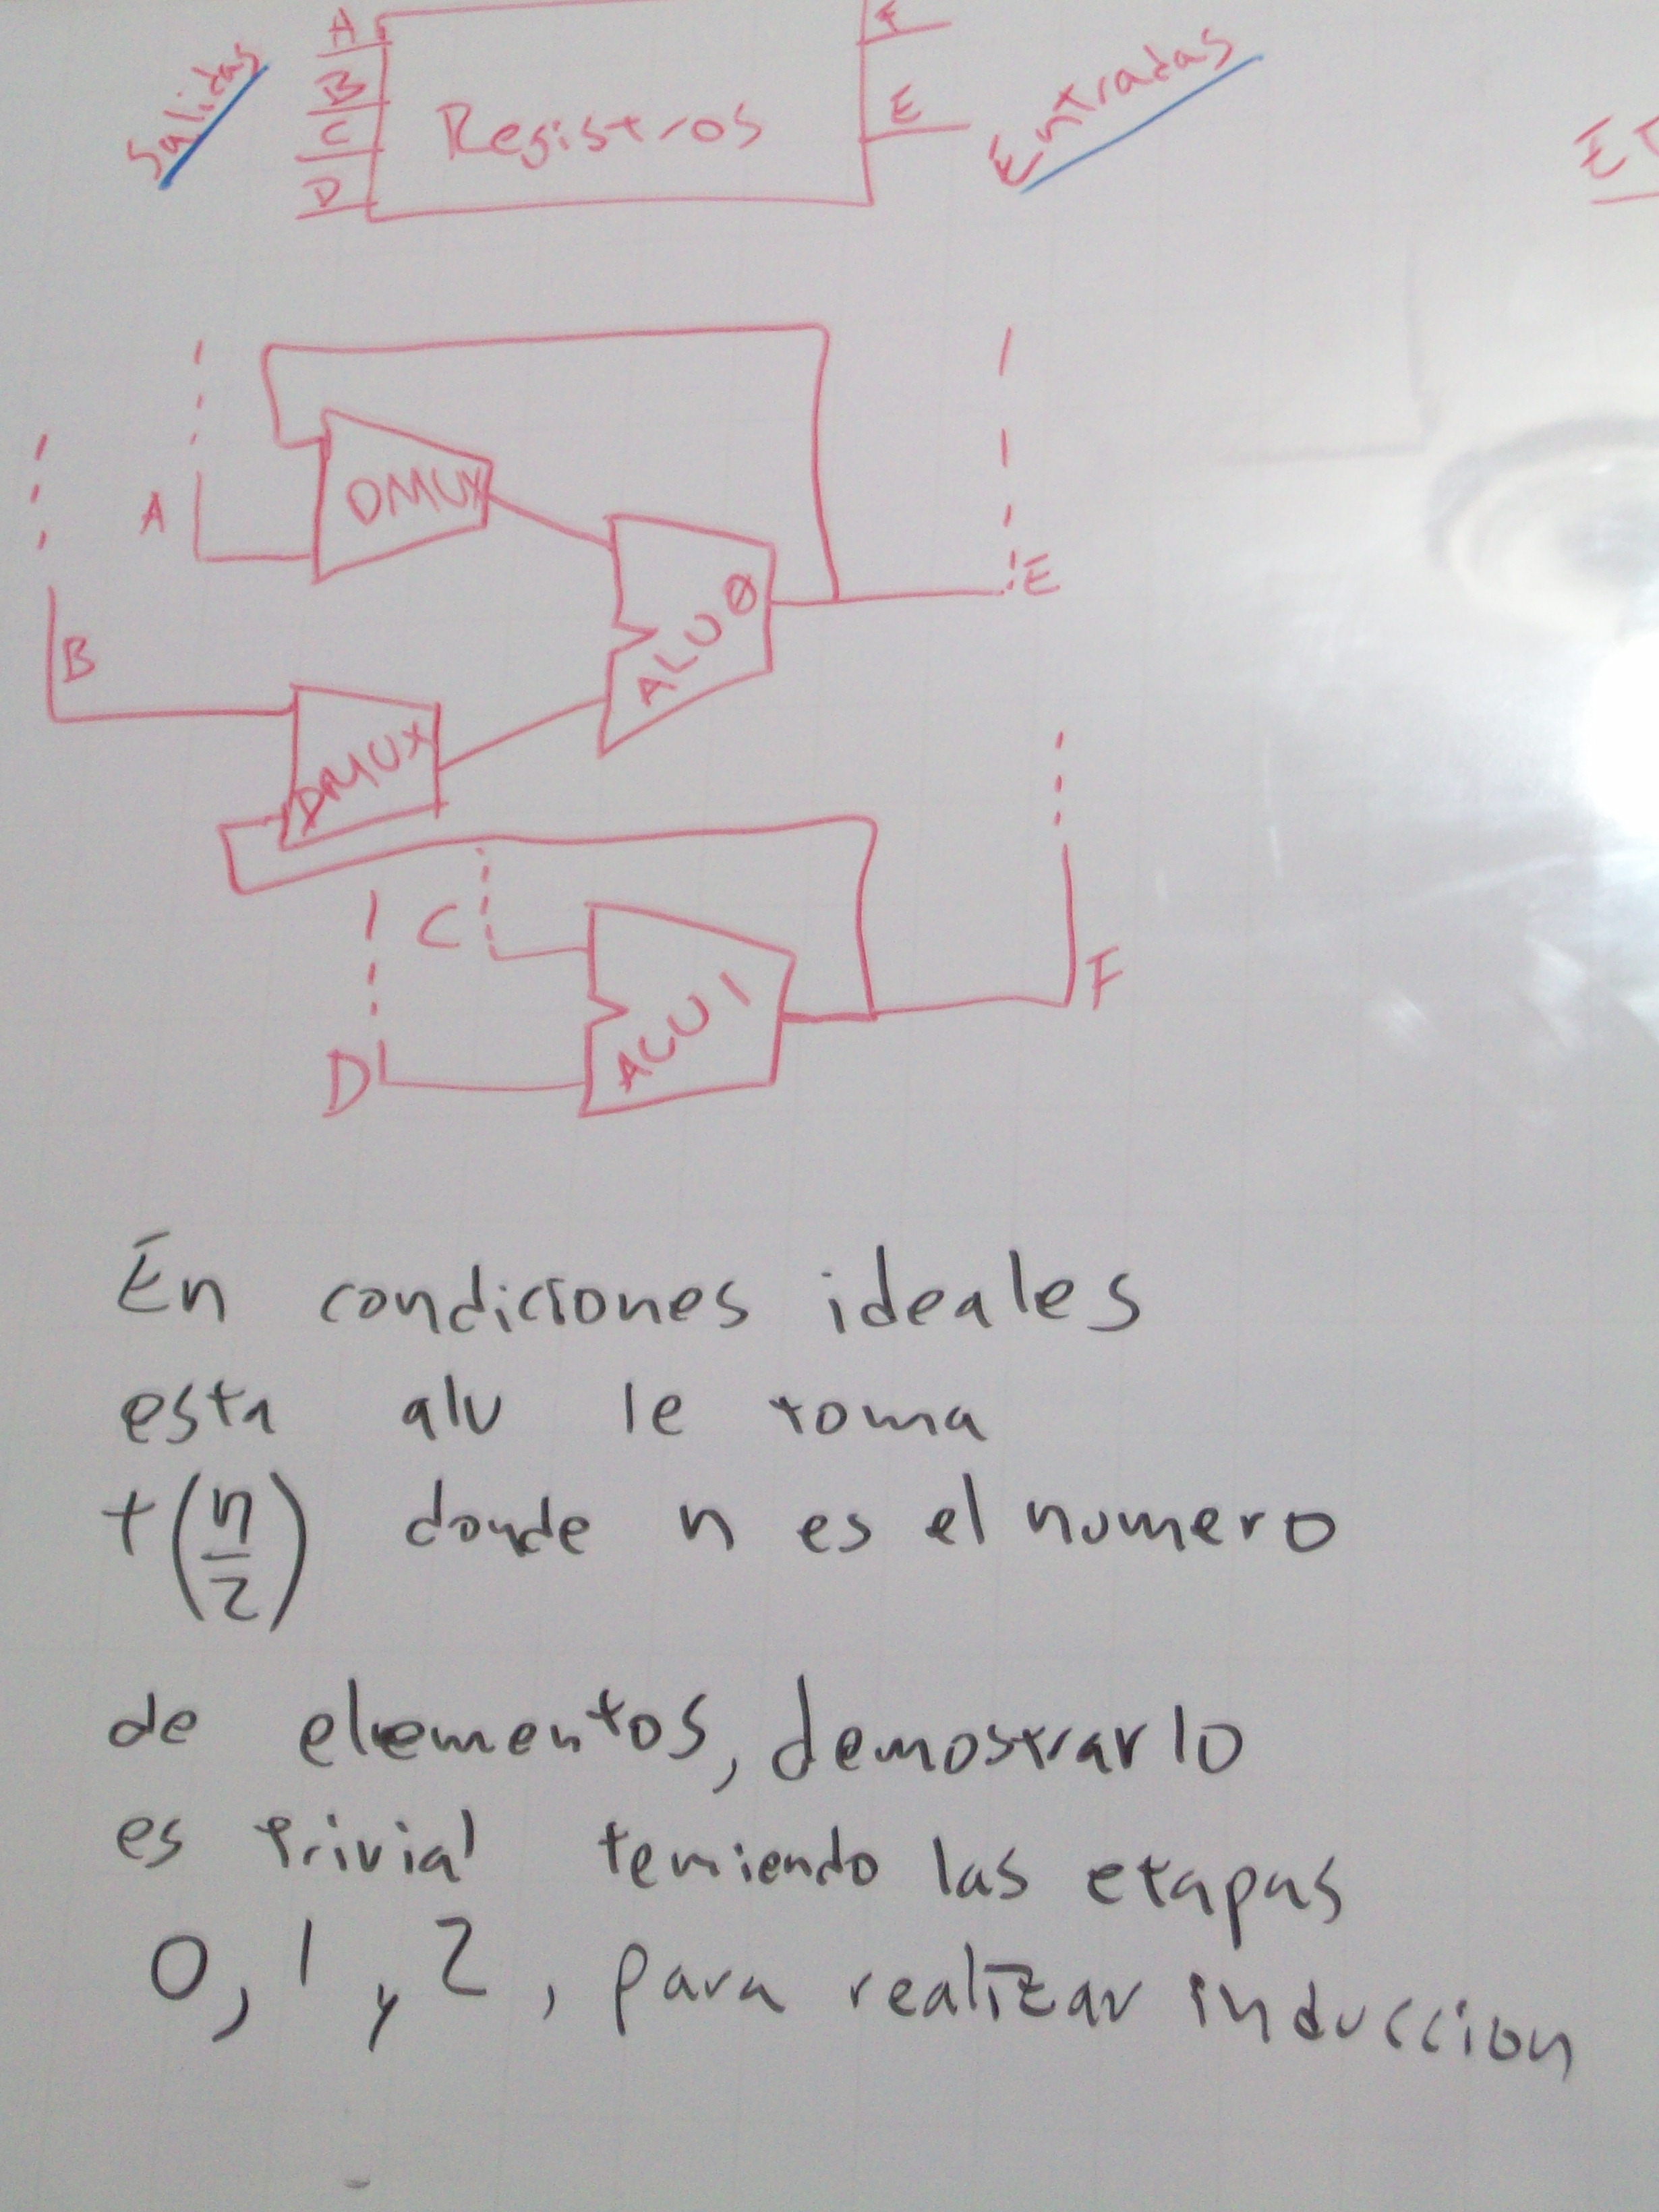
\includegraphics[scale=0.15]{1.jpg}
%	        %\caption{}
%	      \end{figure}

	

	
	Si nos remitimos al diseño de algoritmos nos damos cuenta que por mas que intentemos reducir el orden del algoritmo, tenemos que luchar contra el hecho de que el espacio que estamos atacando es del tamaño $n-1$ (son n elementos por lo tanto $n-1$ sumas), ahora lo único que queda para bajar la complejidad $O(n)$ (es lineal) es paralelizar operaciones, lo cual no nos genera reducción de complejidad sino en tiempo de computo, lo que quiere decir que la constante que absorbe el Big-O  es más pequeña. Ahora bien nos podemos dar facilmente cuenta que la reducción de la constante es dependiente del número de procesos que podamos ejecutar en paralelo, es más estando de la forma $1/k$ donde $k$ es el número de procesos en paralelo, para nuestro caso número de ALUs, y si no es tan claro podemos hacer dos inducciones para probarlo una para probar que con $k$ el tiempo se reduce en $1/k$ y otra para probar que sirver para cualquier $k>=1$.

	

	      
	      
	      
	\section{Tareas por realizar}
	Lista de las actividades que faltan para terminar la práctica y
	que además serían interesantes realizar:
	\begin{itemize}
	\item Montar el juego de señales
	\item Procesador.
	\item Logisim.
	\end{itemize}
	      \pagebreak 
	      
	      
	            \pagebreak 
		            		
	            \pagebreak 
	                                           
%	                        
%	       \begin{figure}[ht]
%	        \centering
%	        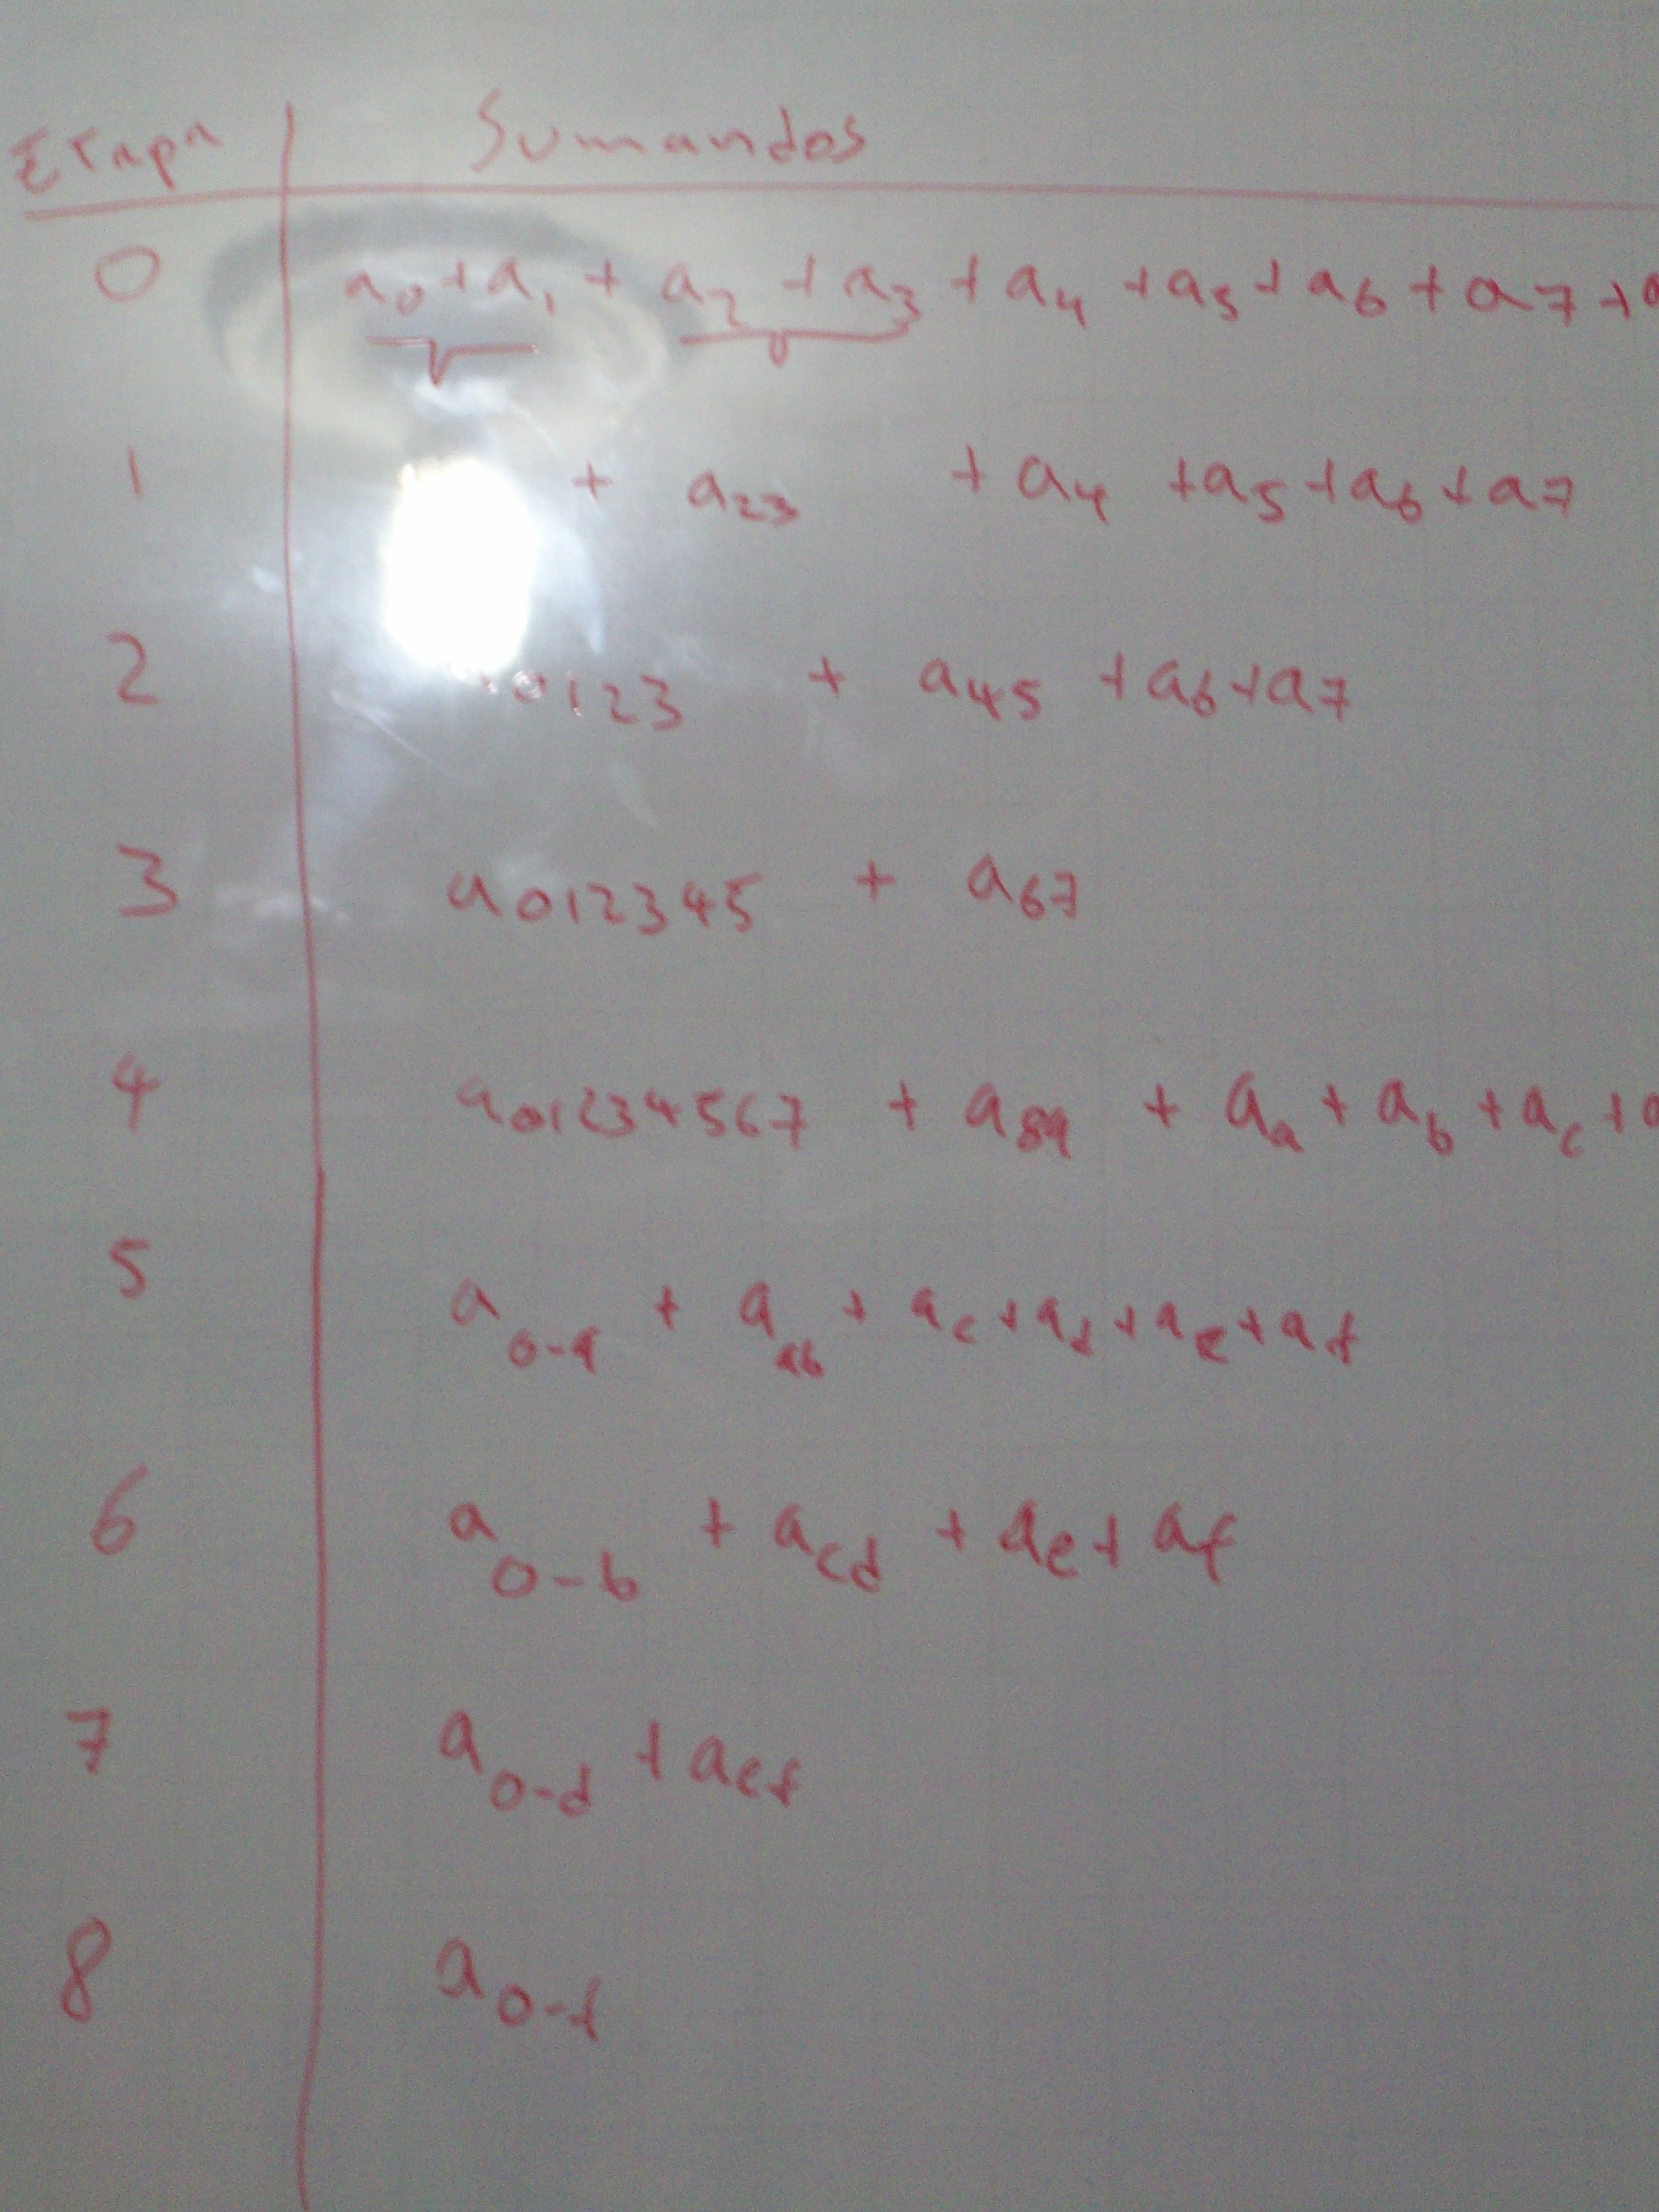
\includegraphics[scale=0.12]{2.jpg}
%	        %\caption{}
%	      \end{figure}
%	                        
	\end{document}